\section{การออกแบบส่วนโครงสร้างระบบฐานข้อมูล (Database Schema)}

การออกแบบส่วนโครงสร้างระบบฐานข้อมูล (Database Schema) จะแสดงในรูปแบบ UML Class Diagram และมีรายละเอียดดังนี้
\subsection{ฐานข้อมูลในคอลเล็กชัน users}
\begin{figure}
    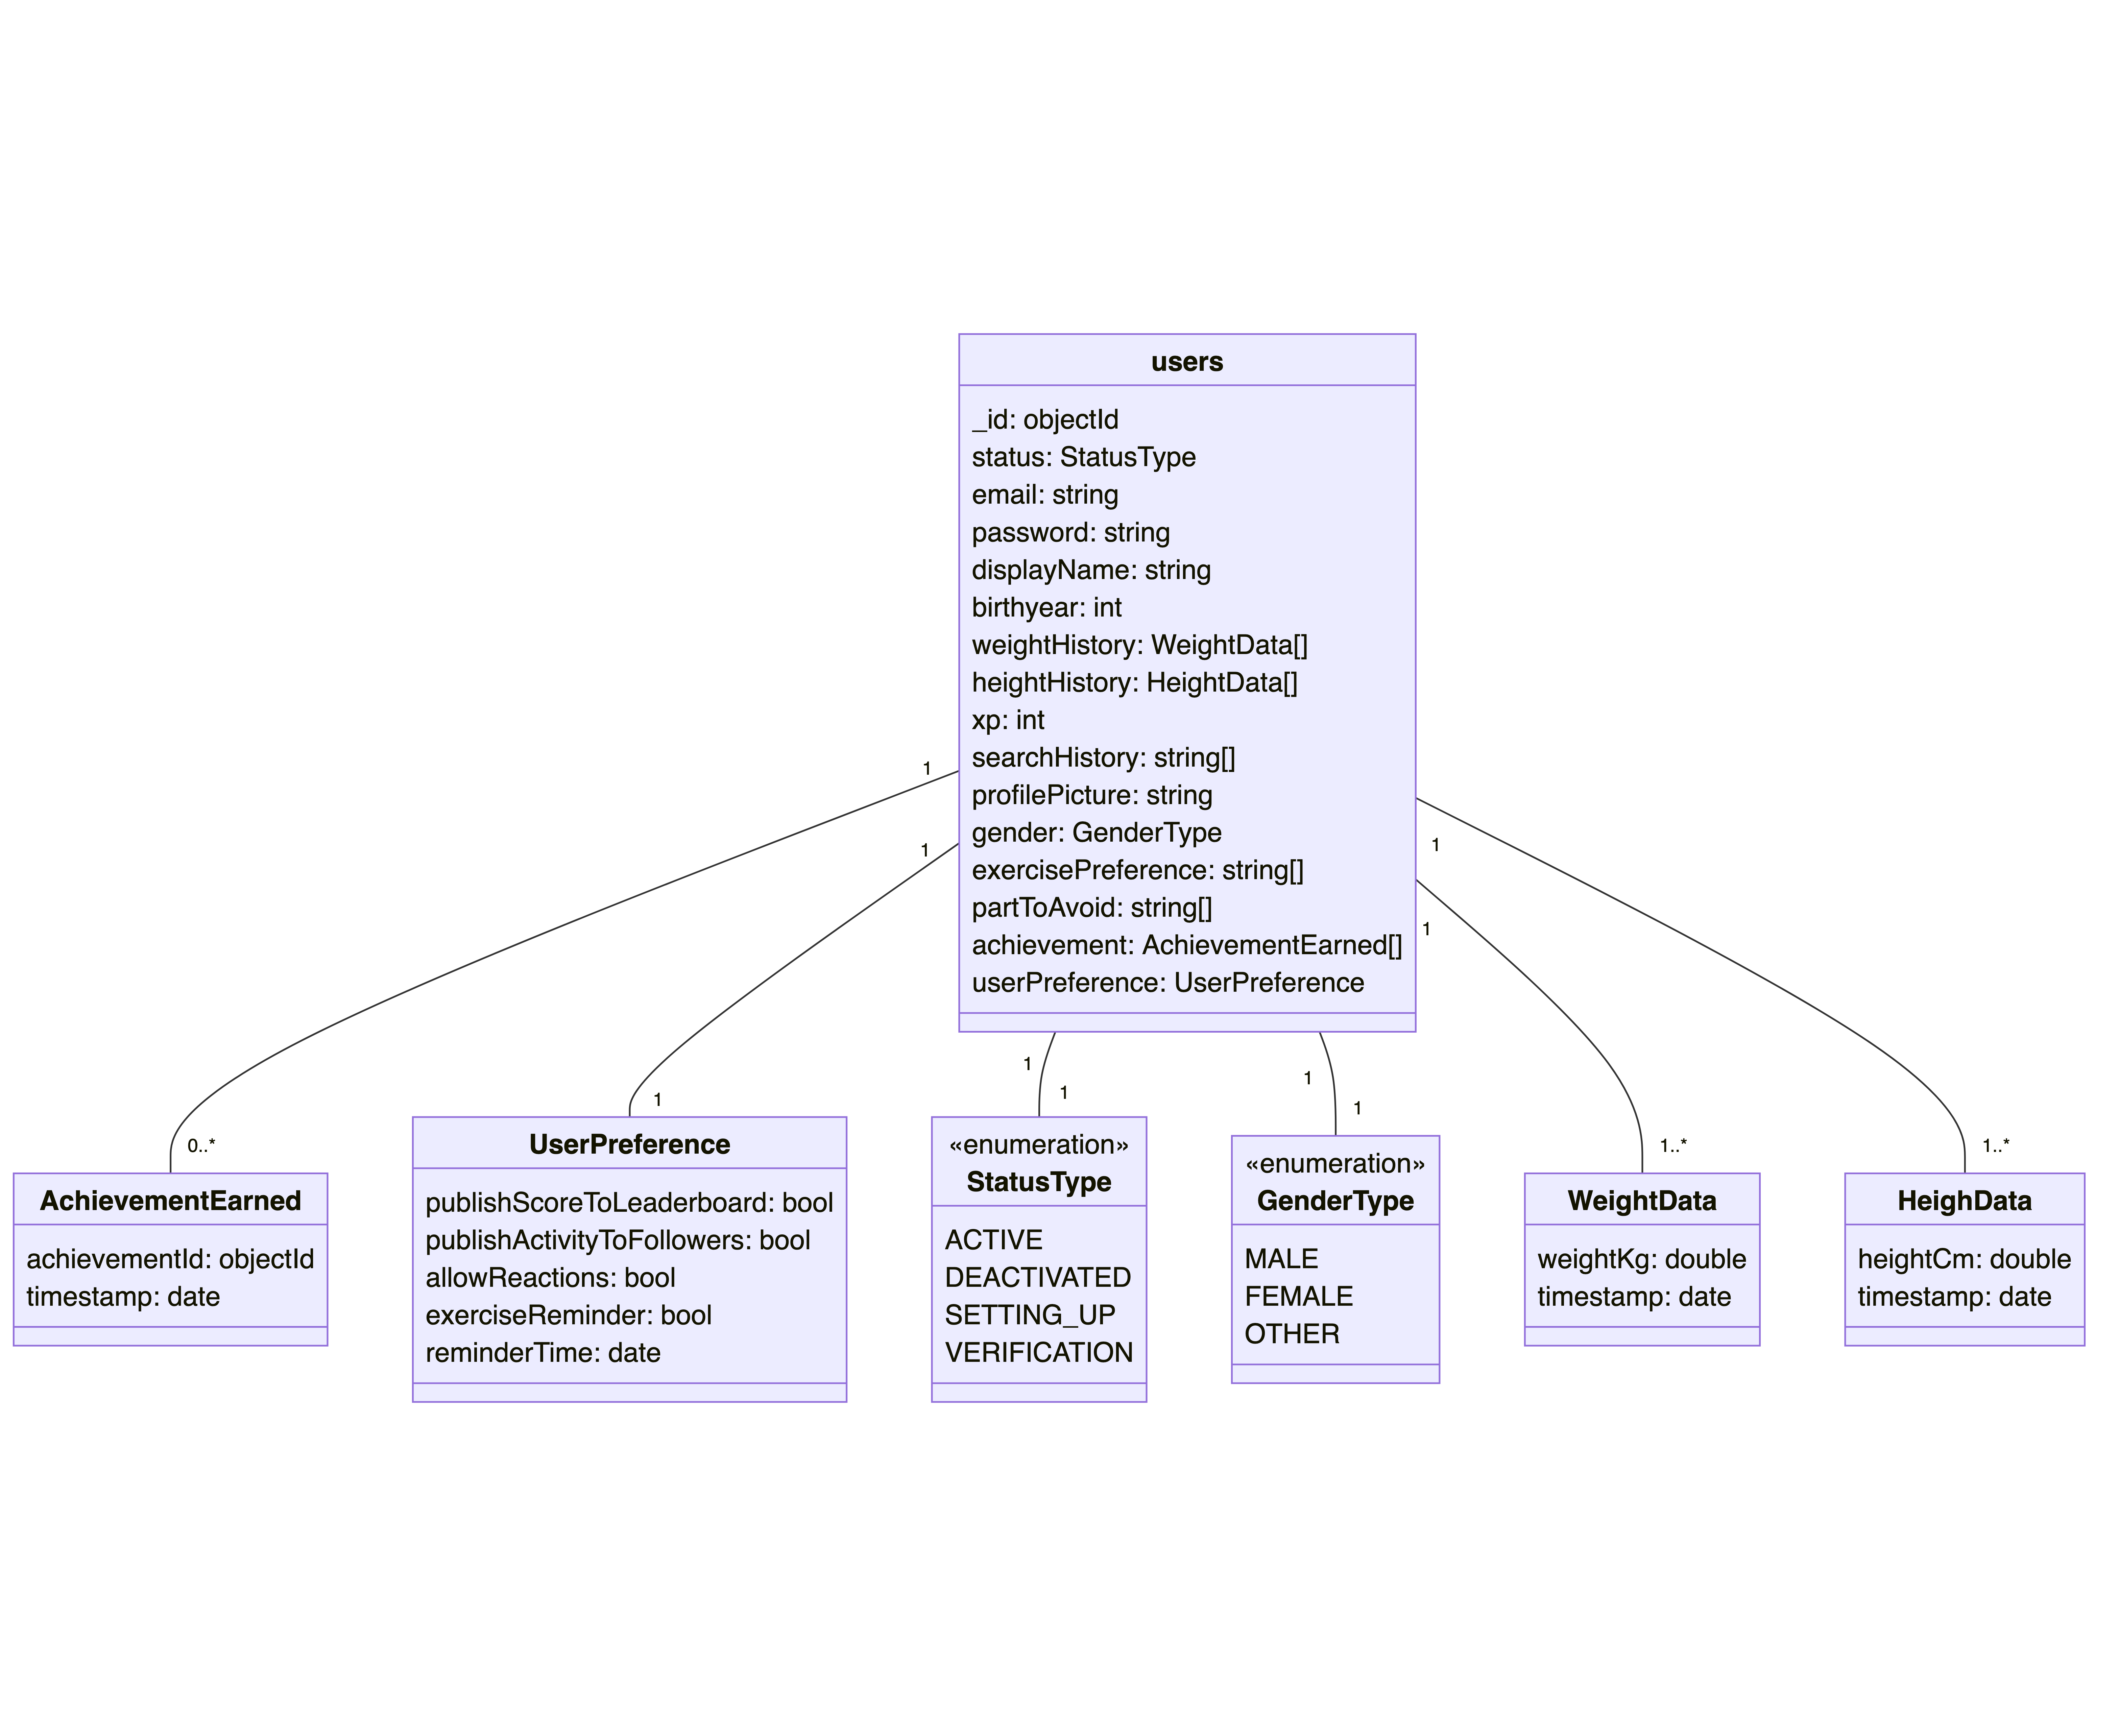
\includegraphics[width=\textwidth]{chapter_3/database/users}
    \caption{แผนภาพยูสเคสในคอลเล็กชัน users}
\end{figure}
\begin{table}
    \caption{รายละเอียดฐานข้อมูลในคอลเล็กชัน users}
    \begin{tabularx}{\textwidth}{ | l | l | X | }
        \hline
        \bf ชื่อแอตทริบิวต์ & \bf ชนิดตัวแปร & \bf รายละเอียด \\\hline
        \_ id & objectId & ID ของ document ในคอลเล็กชัน users\\\hline
        status & StatusType & สถานะของบัญชีผู้ใช้\\\hline
        email & string & อีเมลของผู้ใช้\\\hline
        password & string & รหัสผ่านของผู้ใช้\\\hline
        displayName & string & ชื่อ Display Name ของผู้ใช้\\\hline
        birthyear & int & ปีเกิดของผู้ใช้\\\hline
        weightHistory & WeightData[] & ประวัติน้ำหนักของผู้ใช้\\\hline
        heightHistory & HeightData[] & ประวัติส่วนสูงของผู้ใช้\\\hline
        xp & int & คะแนนของผู้ใช้\\\hline
        profilePicture & string & URL รูปภาพโปรไฟล์ของผู้ใช้\\\hline
        gender & GenderType & เพศของผู้ใช้\\\hline
        exercisePreference & string[] & รายการประเภทการออกกำลังกายที่ชอบ\\\hline
        partToAvoid & string[] & รายการสัดส่วนของผู้ใช้ที่ต้องการหลีกเลี่ยง\\\hline
        userPreference & UserPreference & ข้อมูลการตั้งค่าของผู้ใช้\\\hline
    \end{tabularx}
\end{table}

\begin{table}
    \caption{รายละเอียดชนิดตัวแปร AchievementEarned}
    \begin{tabularx}{\textwidth}{ | l | l | X | }
        \hline
        \bf ชื่อแอตทริบิวต์ & \bf ชนิดตัวแปร & \bf รายละเอียด \\\hline
        achievementId & objectId & ID ของเหรียญรางวัลเสมือน\\\hline
        timestamp & date & วันและเวลาที่ผู้ใช้ได้รับเหรียญ\\\hline 
    \end{tabularx}
\end{table}

\begin{table}
    \caption{รายละเอียดชนิดตัวแปร UserPreference}
    \begin{tabularx}{\textwidth}{ | l | l | X | }
        \hline
        \bf ชื่อแอตทริบิวต์ & \bf ชนิดตัวแปร & \bf รายละเอียด \\\hline
        publishScoreToLeaderboard & bool & เผยแพร่คะแนนของผู้ใช้บนตารางลีดเดอร์บอร์ด\\\hline
        publishActivityToFollowers & bool & เผยแพร่กิจกรรมของผู้ใช้ไปยังคนที่กำลังติดตามผู้ใช้\\\hline
        allowReactions & bool & ให้ผู้อื่นสามารถกด Reaction กับกิจกรรมได้\\\hline
        exerciseReminder & bool & การแจ้งเตือนให้ออกกำลังกาย\\\hline
        reminderTime & date & เวลาที่ผู้ใช้ต้องการให้เตือนเพื่อออกกำลังกาย\\\hline
    \end{tabularx}
\end{table}

\begin{table}
    \caption{รายละเอียด Enumeration StatusType}
    \begin{tabularx}{\textwidth}{ | l | X | }
        \hline
        \bf ชื่อแอตทริบิวต์ & \bf รายละเอียด \\\hline
        ACTIVE & บัญชีผู้ใช้มีสถานะปกติ\\\hline
        DEACTIVATED & บัญชีผู้ใช้มีสถานะปิดบัญชี\\\hline
        SETTING\_UP & บัญชีผู้ใช้มีสถานะกำลังอยู่ในขั้นตอนการตั้งค่าผู้ใช้ใหม่\\\hline
        VERIFICATION & บัญชีผู้ใช้มีสถานะกำลังรอการยืนยันอีเมล\\\hline
    \end{tabularx}
\end{table}

\begin{table}
    \caption{รายละเอียด Enumeration GenderType}
    \begin{tabularx}{\textwidth}{ | l | X | }
        \hline
        \bf ชื่อแอตทริบิวต์ & \bf รายละเอียด \\\hline
        MALE & เพศของผู้ใช้คือเพศชาย\\\hline
        FEMALE & เพศของผู้ใช้คือเพศหญิง\\\hline
        OTHER & เพศของผู้ใช้คืออื่น ๆ\\\hline
    \end{tabularx}
\end{table}

\begin{table}
    \caption{รายละเอียดชนิดตัวแปร WeightData}
    \begin{tabularx}{\textwidth}{ | l | l | X | }
        \hline
        \bf ชื่อแอตทริบิวต์ & \bf ชนิดตัวแปร & \bf รายละเอียด \\\hline
        weightKg & double & น้ำหนักของผู้ใช้ (หน่วยกิโลกรัม)\\\hline
        timestamp & date & วันที่และเวลาที่ผู้ใช้กรอกข้อมูล\\\hline
    \end{tabularx}
\end{table}

\begin{table}
    \caption{รายละเอียดชนิดตัวแปร HeightData}
    \begin{tabularx}{\textwidth}{ | l | l | X | }
        \hline
        \bf ชื่อแอตทริบิวต์ & \bf ชนิดตัวแปร & \bf รายละเอียด \\\hline
        heightCm & double & ส่วนสูงของผู้ใช้ (หน่วยเซนติเมตร)\\\hline
        timestamp & date & วันที่และเวลาที่ผู้ใช้กรอกข้อมูล\\\hline
    \end{tabularx}
\end{table}

\subsection{ฐานข้อมูลในคอลเล็กชัน courses}
\begin{figure}
    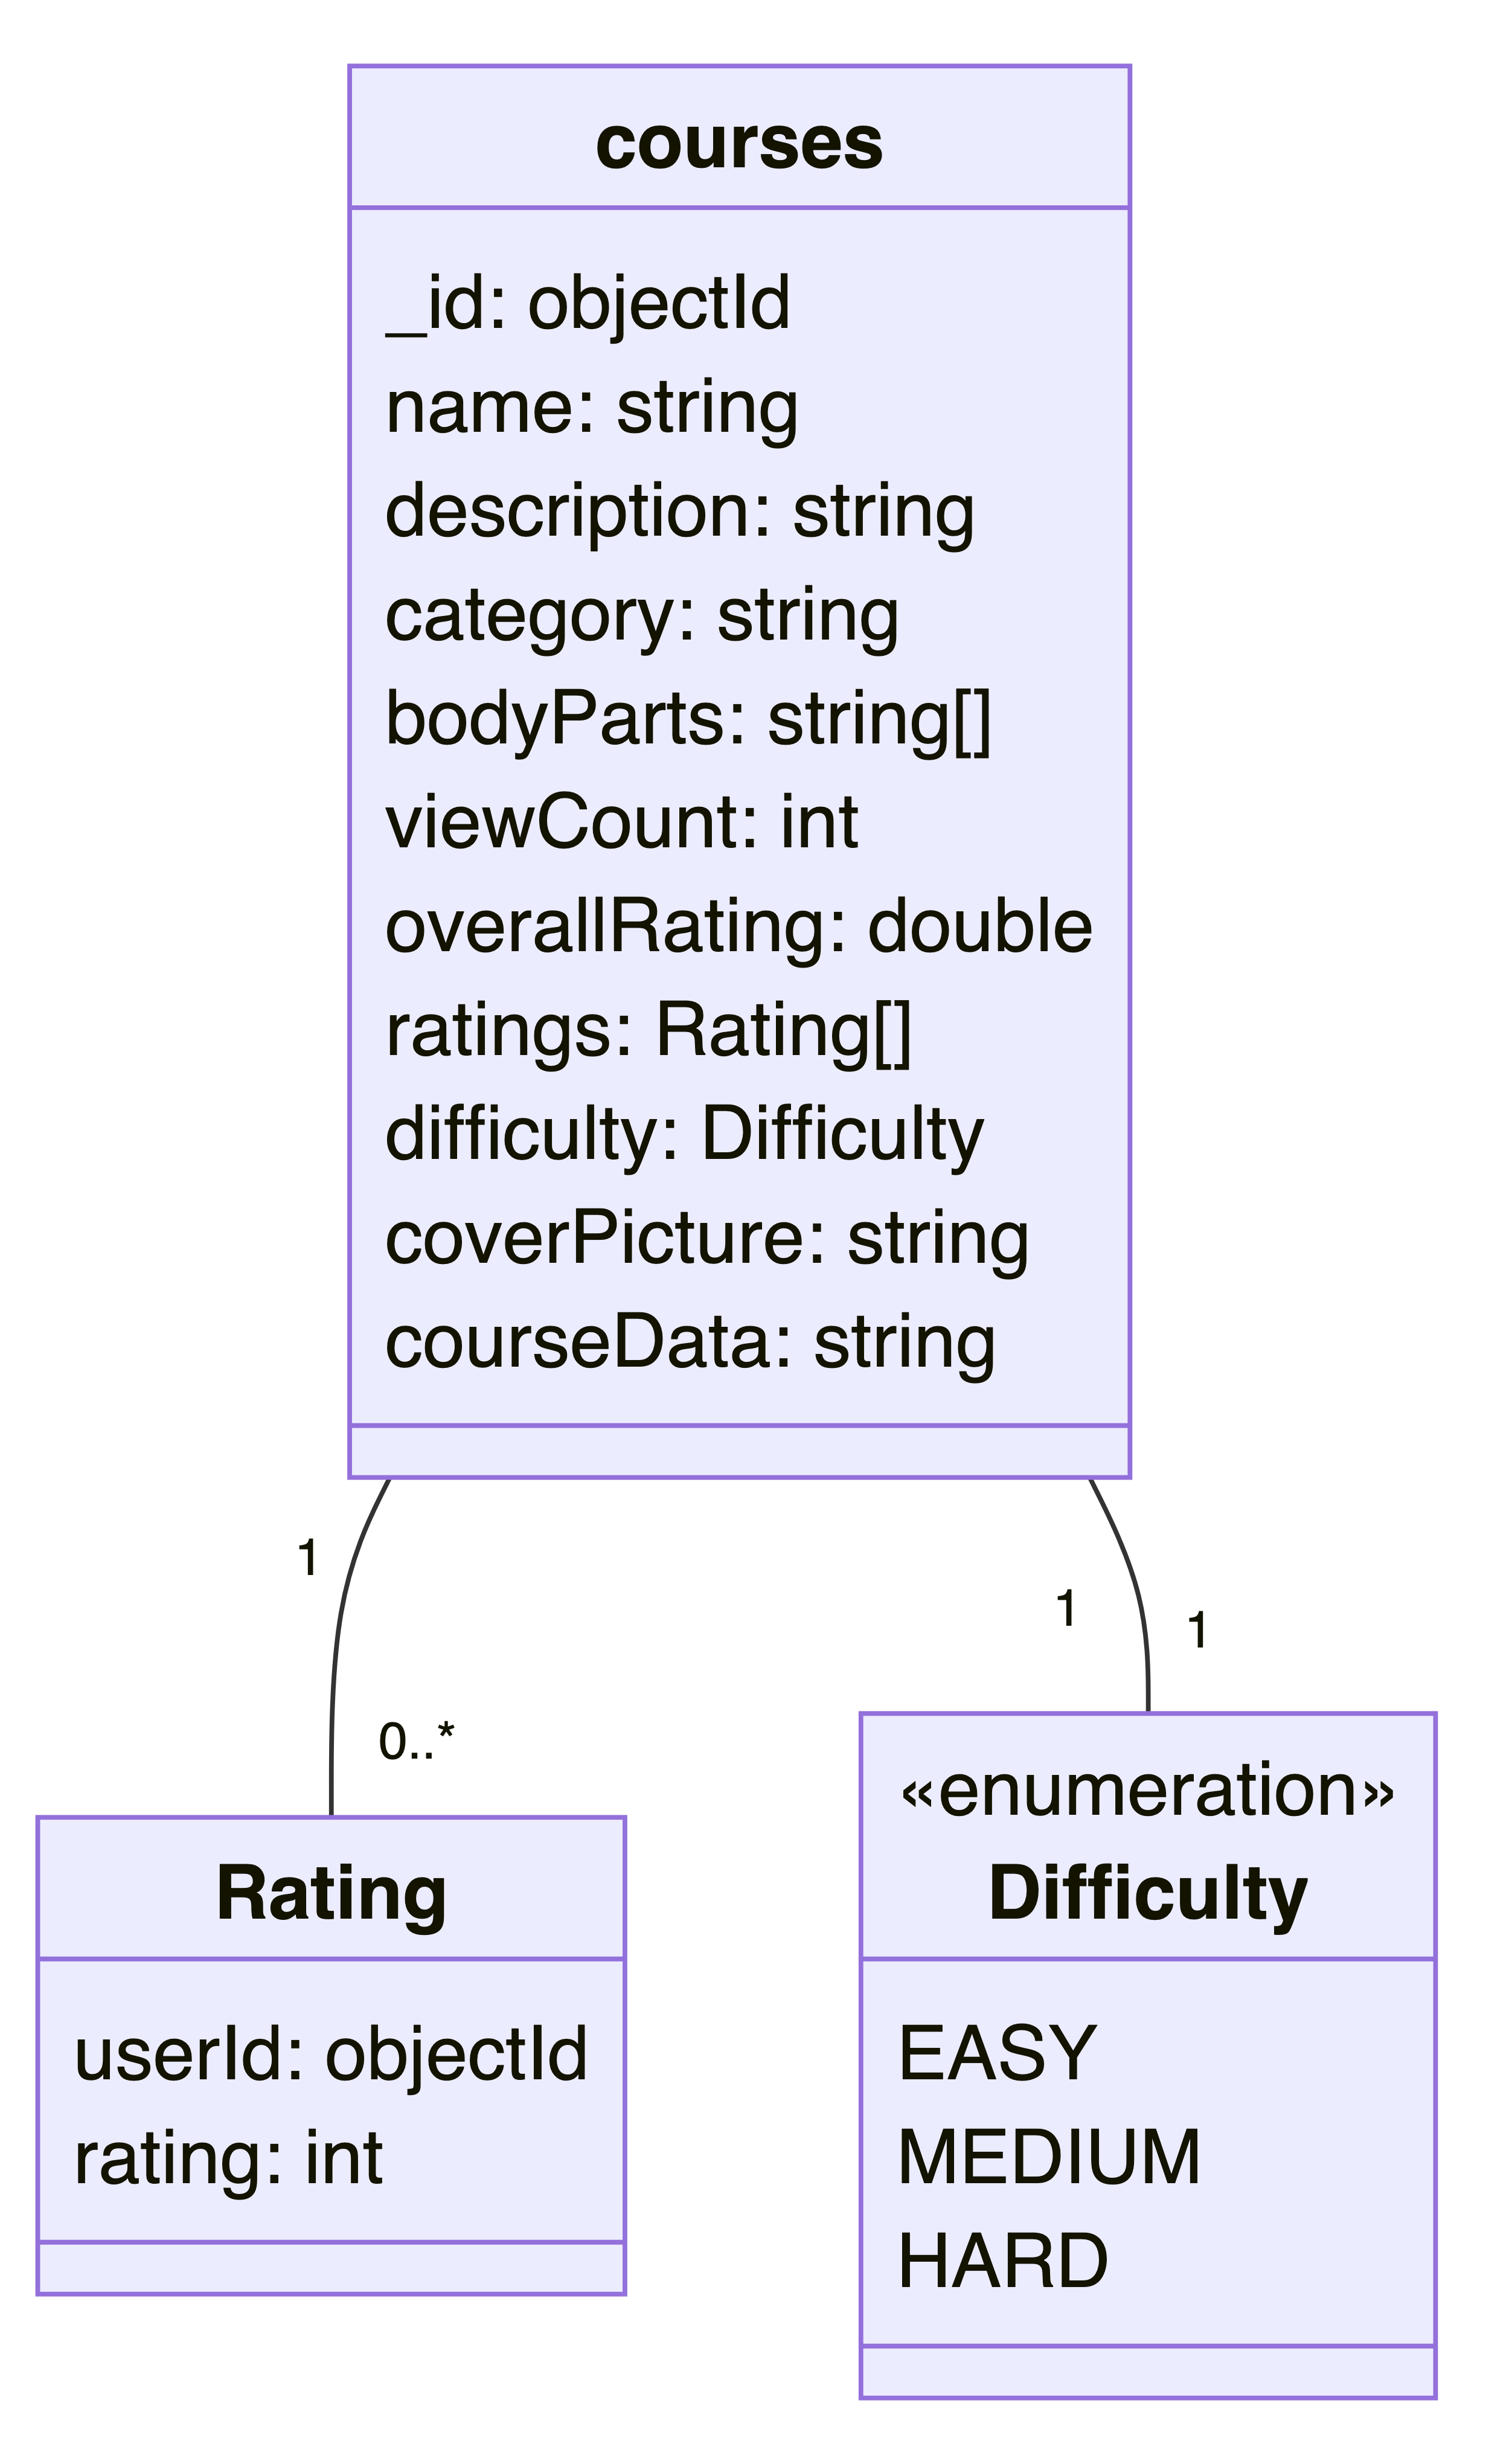
\includegraphics[width=8cm]{chapter_3/database/courses}
    \caption{แผนภาพยูสเคสในคอลเล็กชัน courses}
\end{figure}

\begin{table}
    \caption{รายละเอียดฐานข้อมูลในคอลเล็กชัน courses}
    \begin{tabularx}{\textwidth}{ | l | l | X | }
        \hline
        \bf ชื่อแอตทริบิวต์ & \bf ชนิดตัวแปร & \bf รายละเอียด \\\hline
        \_id & objectId & ID ของ document ในคอลเล็กชัน courses\\\hline
        name & string & ชื่อคอร์ส\\\hline
        description & string & คำอธิบายของคอร์ส\\\hline
        category & string & หมวดหมู่คอร์ส\\\hline
        bodyParts & string[] & ส่วนของร่างกายที่ต้องใช้\\\hline
        viewCount & int & จำนวนการเข้าดูคอร์สนี้\\\hline
        overallRating & double & คะแนนเฉลี่ยของคอร์สนี้\\\hline
        rating & Rating[] & รายการของผู้ใช้ที่ให้คะแนนกับคอร์สนี้\\\hline
        difficulty & Difficulty & ความยาก-ง่ายของคอร์ส\\\hline
        coverPicture & string & URL รูปภาพหน้าปกคอร์ส\\\hline
        courseData & string & URL ไฟล์ข้อมูลท่าทางการออกกำลังกาย\\\hline
    \end{tabularx}
\end{table}

\begin{table}
    \caption{รายละเอียดชนิดตัวแปร Rating}
    \begin{tabularx}{\textwidth}{ | l | l | X | }
        \hline
        \bf ชื่อแอตทริบิวต์ & \bf ชนิดตัวแปร & \bf รายละเอียด \\\hline
        userId & objectId & ID ของผู้ใช้ที่ให้คะแนน\\\hline
        rating & int & คะแนนที่ผู้ใช้ให้\\\hline
    \end{tabularx}
\end{table}

\begin{table}
    \caption{รายละเอียด Enumeration Difficulty}
    \begin{tabularx}{\textwidth}{ | l | X | }
        \hline
        \bf ชื่อแอตทริบิวต์ & \bf รายละเอียด \\\hline
        EASY & คอร์สระดับง่าย\\\hline
        MEDIUM & คอร์สระดับปานกลาง\\\hline
        HARD & คอร์สระดับยาก\\\hline
    \end{tabularx}
\end{table}

\subsection{ฐานข้อมูลในคอลเล็กชัน achievements}
\begin{figure}
    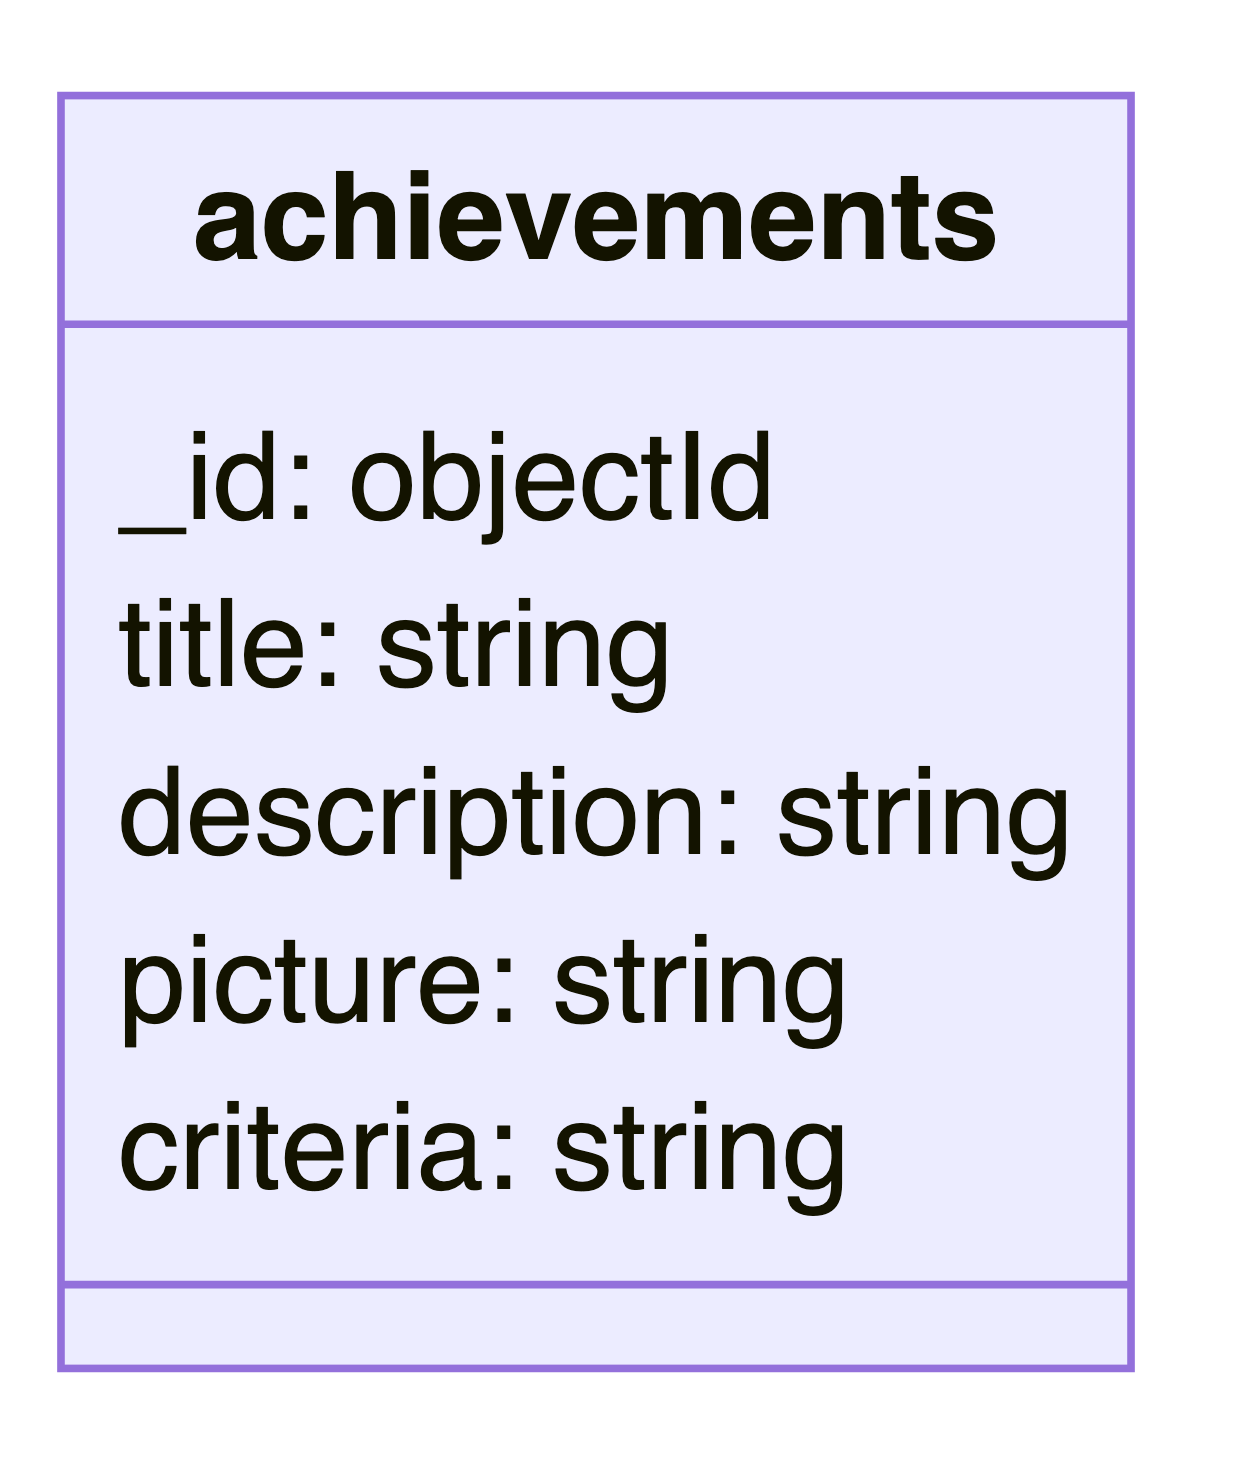
\includegraphics[width=5cm]{chapter_3/database/achievements}
    \caption{แผนภาพยูสเคสในคอลเล็กชัน achievements}
\end{figure}


\begin{table}
    \caption{รายละเอียดฐานข้อมูลในคอลเล็กชัน achievements}
    \begin{tabularx}{\textwidth}{ | l | l | X | }
        \hline
        \bf ชื่อแอตทริบิวต์ & \bf ชนิดตัวแปร & \bf รายละเอียด \\\hline
        \_id & objectId & ID ของเหรียญรางวัลเสมือน\\\hline
        title & string & ชื่อของเหรียญรางวัลเสมือน\\\hline
        description & string & คำอธิบายเหรียญรางวัลเสมือน\\\hline
        picture & string & รูปภาพของเหรียญรางวัลเสมือน\\\hline
        criteria & string & เกณฑ์ต่าง ๆ ของเหรียญรางวัลเสมือน\\\hline
    \end{tabularx}
\end{table}

\subsection{ฐานข้อมูลในคอลเล็กชัน activities}
\begin{figure}
    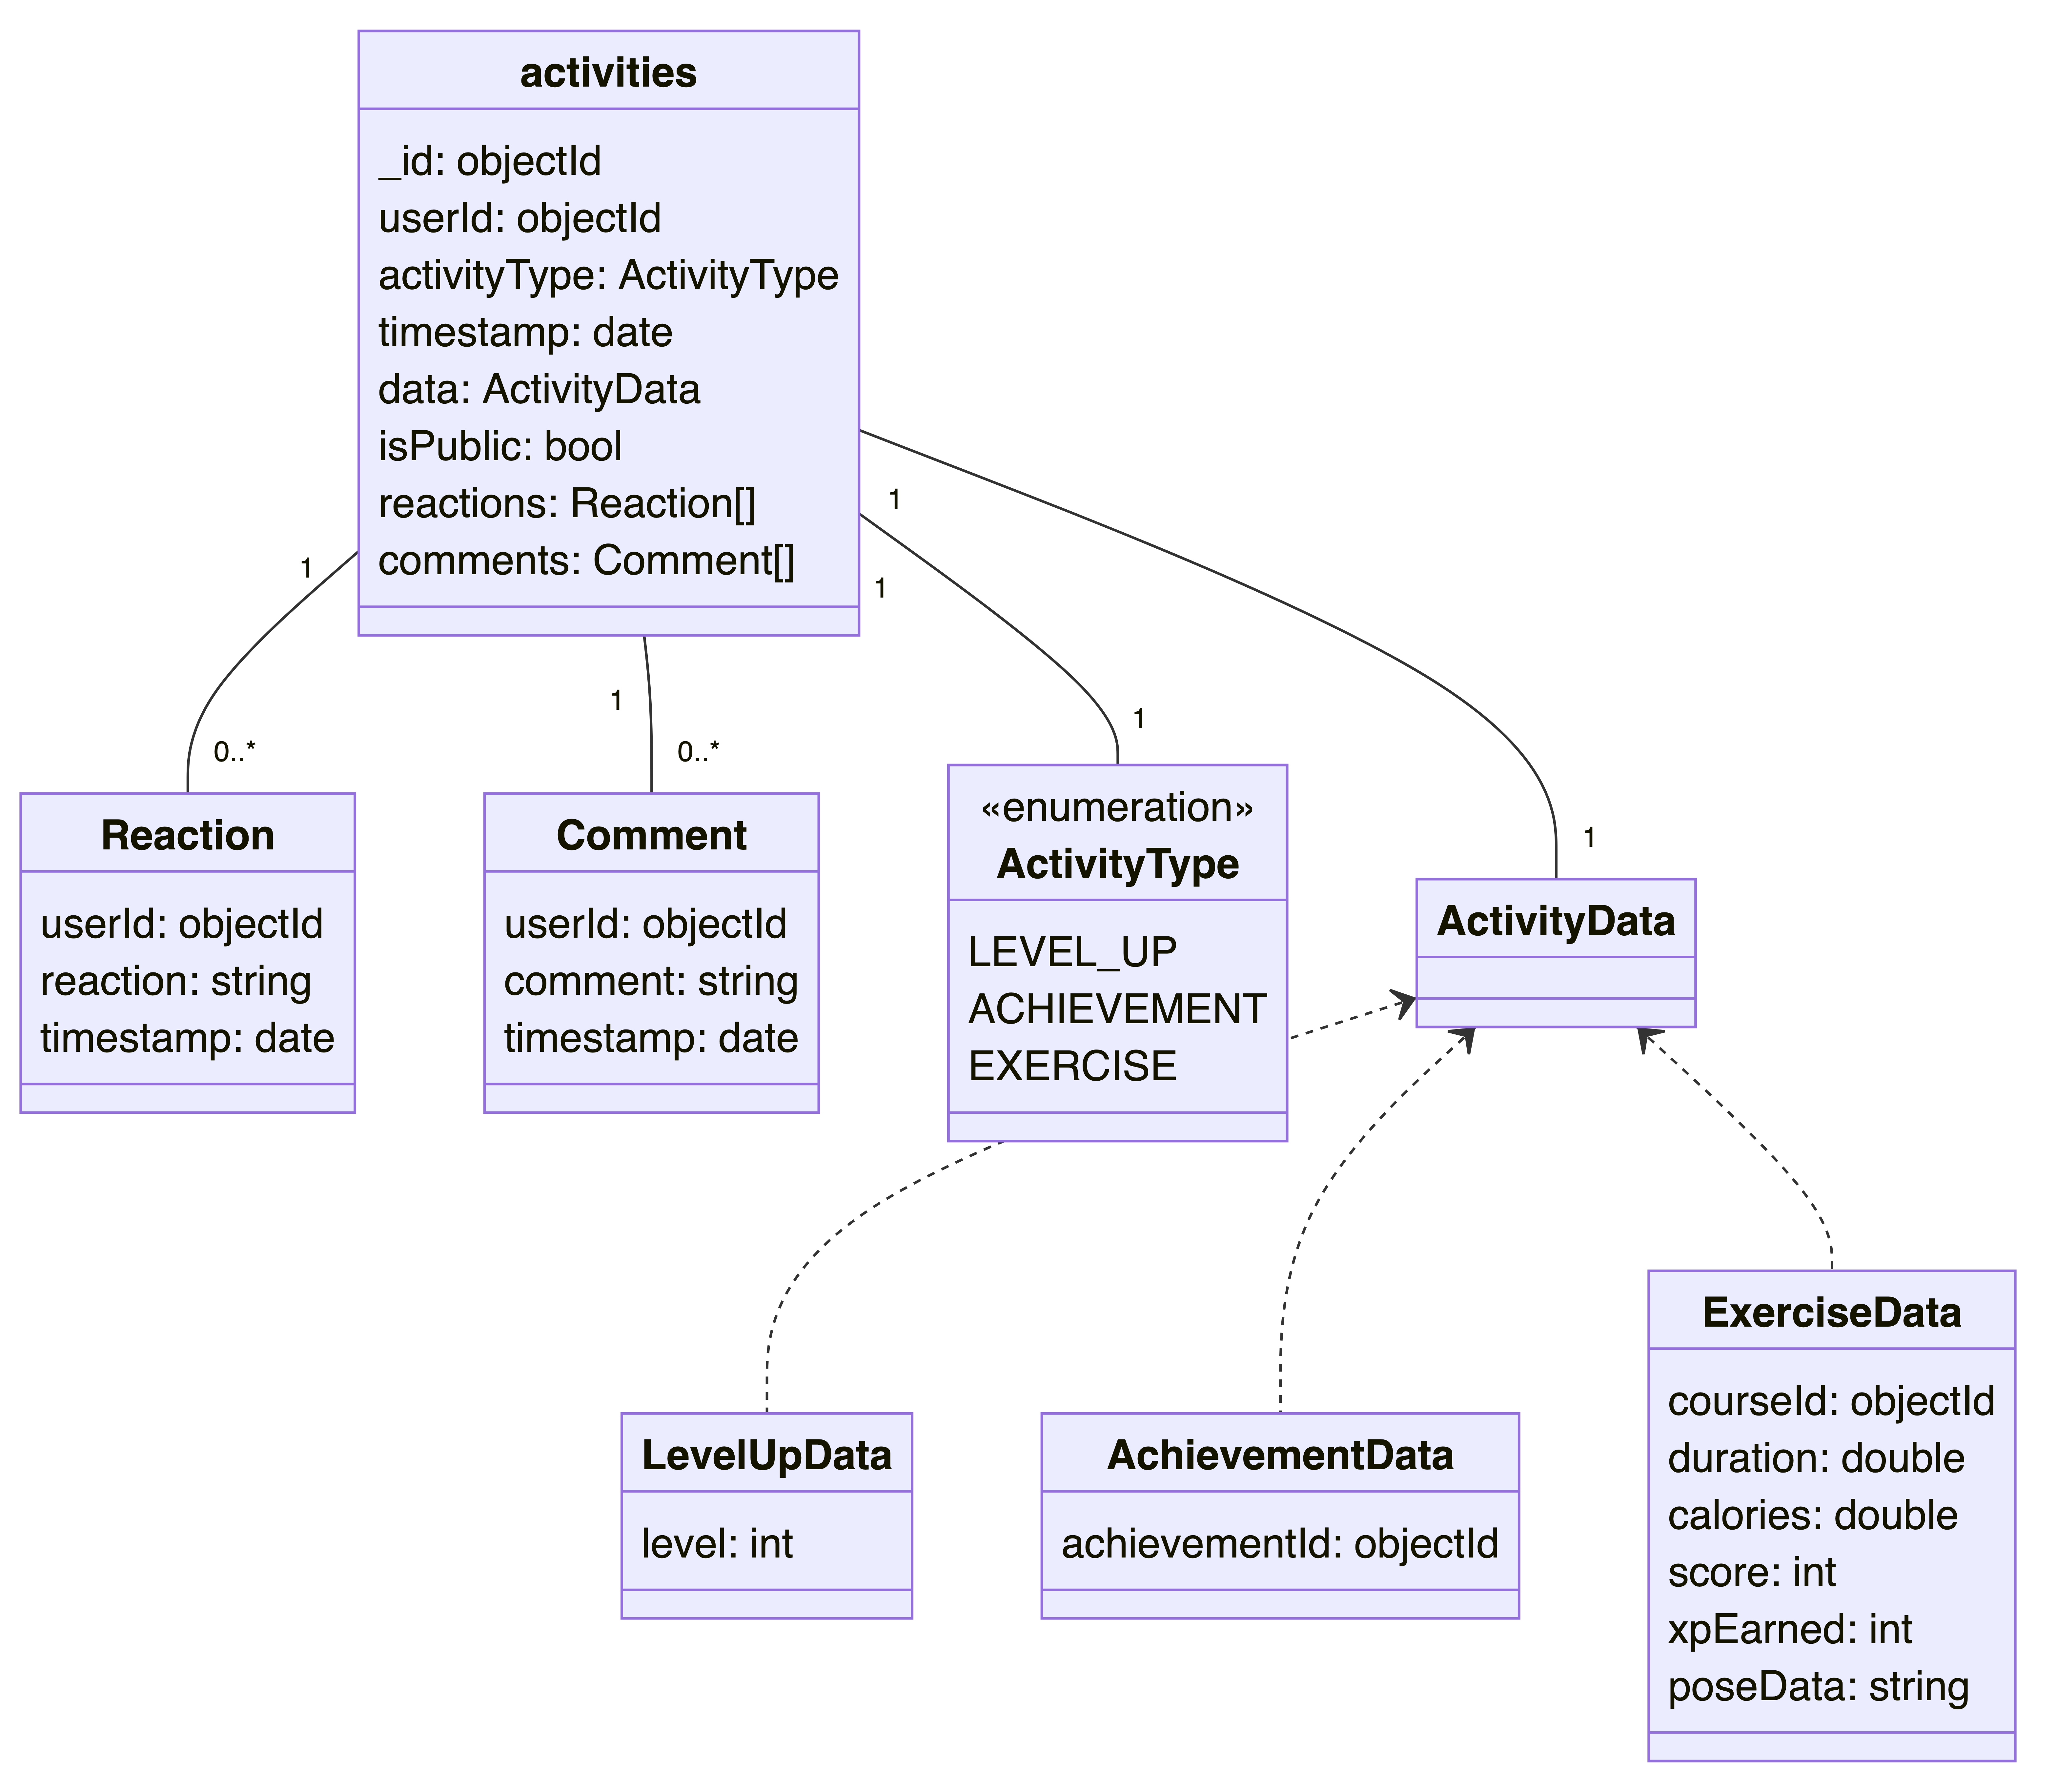
\includegraphics[width=\textwidth]{chapter_3/database/activities}
    \caption{แผนภาพยูสเคสในคอลเล็กชัน activities}
\end{figure}

\begin{table}
    \caption{รายละเอียดฐานข้อมูลในคอลเล็กชัน activities}
    \begin{tabularx}{\textwidth}{ | l | l | X | }
        \hline
        \bf ชื่อแอตทริบิวต์ & \bf ชนิดตัวแปร & \bf รายละเอียด \\\hline
        \_id & objectId & ID ของกิจกรรม\\\hline
        userId & objectId & ID ของผู้ใช้ที่เป็นผู้ทำกิจกรรม\\\hline
        activityType & ActivityType & ประเภทของกิจกรรม\\\hline
        timestamp & date & วันที่และเวลาที่ทำกิจกรรม\\\hline
        data & ActivityData & ข้อมูลรายละเอียดของกิจกรรม\\\hline
        isPublic & bool & ให้กิจกรรมนี้สามารถให้ผู้ที่ติดตามมองเห็นได้หรือไม่\\\hline
        reactions & Reaction[] & รายการผู้ใช้ที่กดแสดงความรู้สึก (Reaction) ต่อกิจกรรมนี้\\\hline
        comments & Comment[] & รายการที่ผู้ใช้แสดงความคิดเห็น (Comment) ต่อกิจกรรมนี้\\\hline
    \end{tabularx}
\end{table}

\begin{table}
    \caption{รายละเอียดชนิดตัวแปร LevelUpData}
    \begin{tabularx}{\textwidth}{ | l | l | X | }
        \hline
        \bf ชื่อแอตทริบิวต์ & \bf ชนิดตัวแปร & \bf รายละเอียด \\\hline
        level & int & ระดับ (Level) ที่ผู้ใช้ได้รับ\\\hline
    \end{tabularx}
\end{table}

\begin{table}
    \caption{รายละเอียดชนิดตัวแปร ExerciseData}
    \begin{tabularx}{\textwidth}{ | l | l | X | }
        \hline
        \bf ชื่อแอตทริบิวต์ & \bf ชนิดตัวแปร & \bf รายละเอียด \\\hline
        courseId & objectId & ID ของคอร์สที่ผู้ใช้ได้ออกกำลังกาย\\\hline
        duration & double & ระยะเวลาที่ผู้ใช้เข้าคอร์ส (นาที)\\\hline
        calories & double & จำนวนแคลอรีที่ผู้ใช้ได้เผาผลาญไป\\\hline
        score & int & คะแนนความถูกต้องในการออกกำลังกายของผู้ใช้ (เป็นช่วงจาก 0 - 100)\\\hline
        xpEarned & int & คะแนนที่ผู้ใช้ได้รับ\\\hline
        poseData & string & URL ไฟล์ข้อมูลท่าทางของผู้ใช้\\\hline
    \end{tabularx}
\end{table}

\begin{table}
    \caption{รายละเอียด Enumeration ActivityType}
    \begin{tabularx}{\textwidth}{ | l | X | }
        \hline
        \bf ชื่อแอตทริบิวต์ & \bf รายละเอียด \\\hline
        LEVEL\_UP & กิจกรรม ประเภทการเลื่อนระดับ\\\hline
        ACHIEVEMENT & กิจกรรม ประเภทที่ได้รับเหรียญรางวัลเสมือน\\\hline
        EXERCISE & กิจกรรม ประเภทการออกกำลังกาย\\\hline
    \end{tabularx}
\end{table}

\begin{table}
    \caption{รายละเอียดชนิดตัวแปร Reaction}
    \begin{tabularx}{\textwidth}{ | l | l | X | }
        \hline
        \bf ชื่อแอตทริบิวต์ & \bf ชนิดตัวแปร & \bf รายละเอียด \\\hline
        \_id & objectId & ID ของกิจกรรม\\\hline
        userId & objectId & ID ของผู้ใช้ที่ได้แสดงความรู้สึก (Reaction)\\\hline
        reaction & string & ชื่อความรู้สึก (Reaction)\\\hline
        timestamp & date & วันที่และเวลาที่ได้กดแสดงความรู้สึก (Reaction)\\\hline
    \end{tabularx}
\end{table}

\begin{table}
    \caption{รายละเอียดชนิดตัวแปร Comment}
    \begin{tabularx}{\textwidth}{ | l | l | X | }
        \hline
        \bf ชื่อแอตทริบิวต์ & \bf ชนิดตัวแปร & \bf รายละเอียด \\\hline
        \_id & objectId & ID ของกิจกรรม\\\hline
        userId & objectId & ID ของผู้ใช้ที่ได้แสดงความคิดเห็น\\\hline
        comment & string & ความคิดเห็นของผู้ใช้\\\hline
        timestamp & date & วันที่และเวลาที่ได้แสดงความคิดเห็น\\\hline
    \end{tabularx}
\end{table}

\subsection{ฐานข้อมูลในคอลเล็กชัน news}
\begin{figure}
    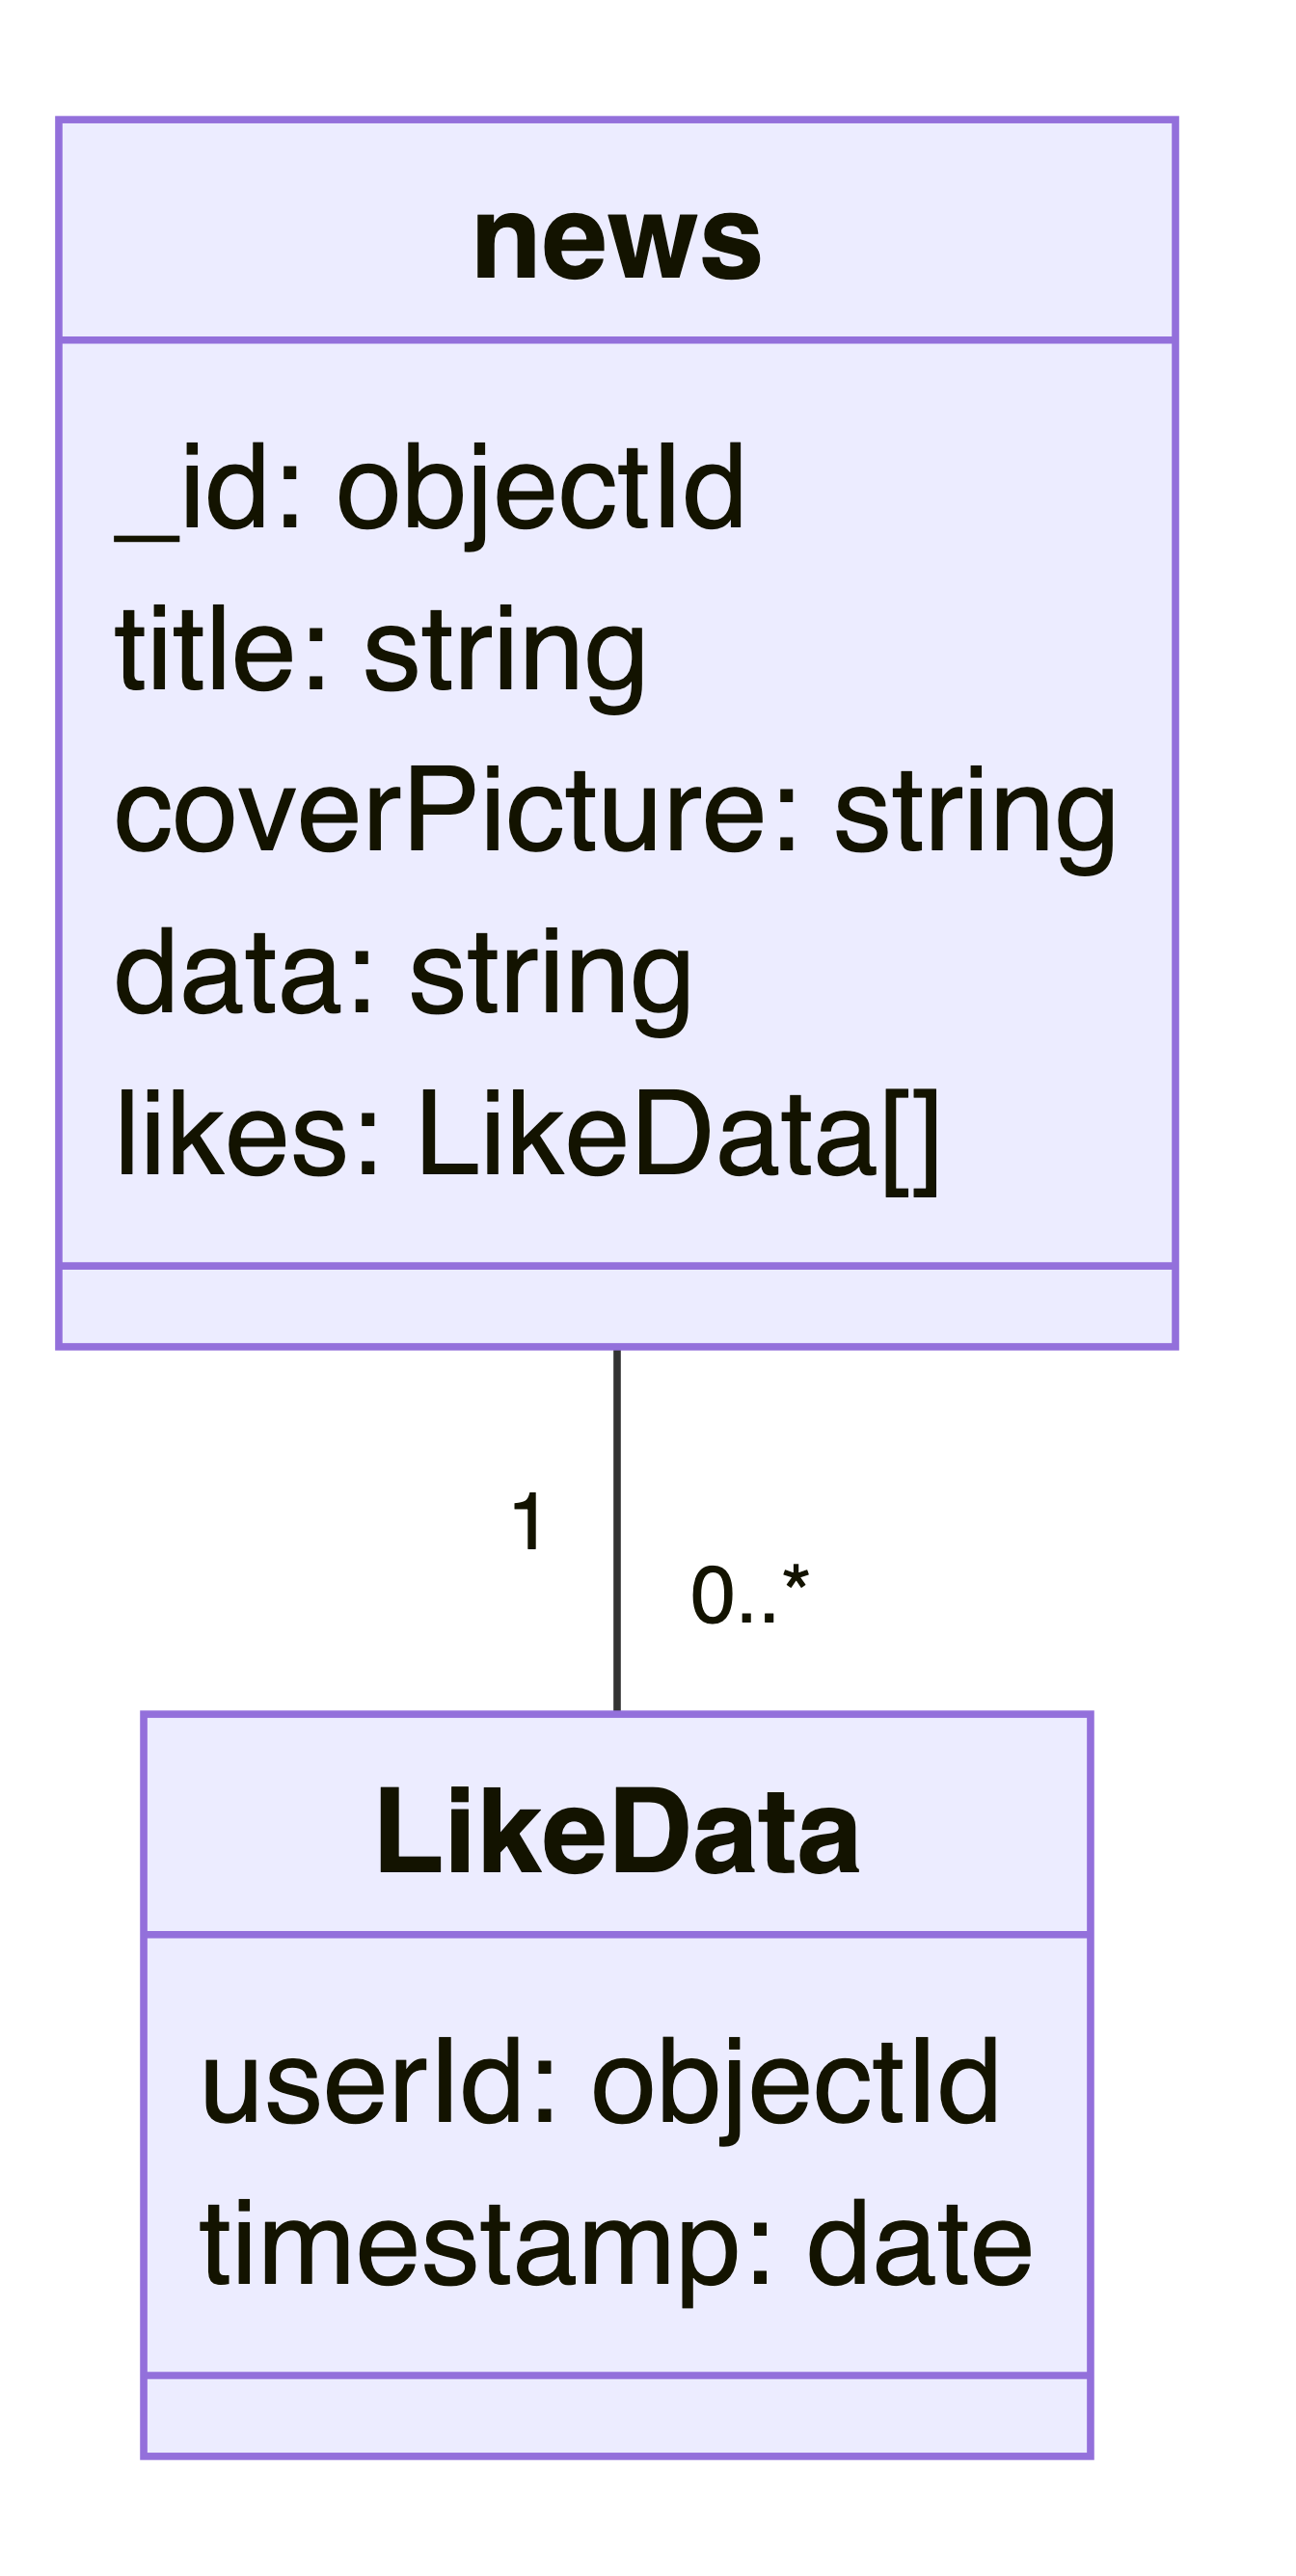
\includegraphics[width=5cm]{chapter_3/database/news}
    \caption{แผนภาพยูสเคสในคอลเล็กชัน news}
\end{figure}

\begin{table}
    \caption{รายละเอียดฐานข้อมูลในคอลเล็กชัน news}
    \begin{tabularx}{\textwidth}{ | l | l | X | }
        \hline
        \bf ชื่อแอตทริบิวต์ & \bf ชนิดตัวแปร & \bf รายละเอียด \\\hline
        \_id & objectId & ID ของข่าวสาร\\\hline
        title & string & หัวเรื่องของข่าวสาร\\\hline
        coverPicture & string & URL รูปภาพหน้าปก\\\hline
        data & string & URL ไฟล์ข้อมูลของข่าวสาร\\\hline
        likes & LikeData[] & รายการผู้ที่กดชื่นชอบข่าว\\\hline
    \end{tabularx}
\end{table}

\begin{table}
    \caption{รายละเอียดชนิดตัวแปร LikeData}
    \begin{tabularx}{\textwidth}{ | l | l | X | }
        \hline
        \bf ชื่อแอตทริบิวต์ & \bf ชนิดตัวแปร & \bf รายละเอียด \\\hline
        userId & objectId & ID ของผู้ใช้\\\hline
        timestamp & date & วันและเวลาที่ผู้ใช้กดชื่นชอบ\\\hline
    \end{tabularx}
\end{table}

\subsection{ฐานข้อมูลในคอลเล็กชัน sections}
\begin{figure}
    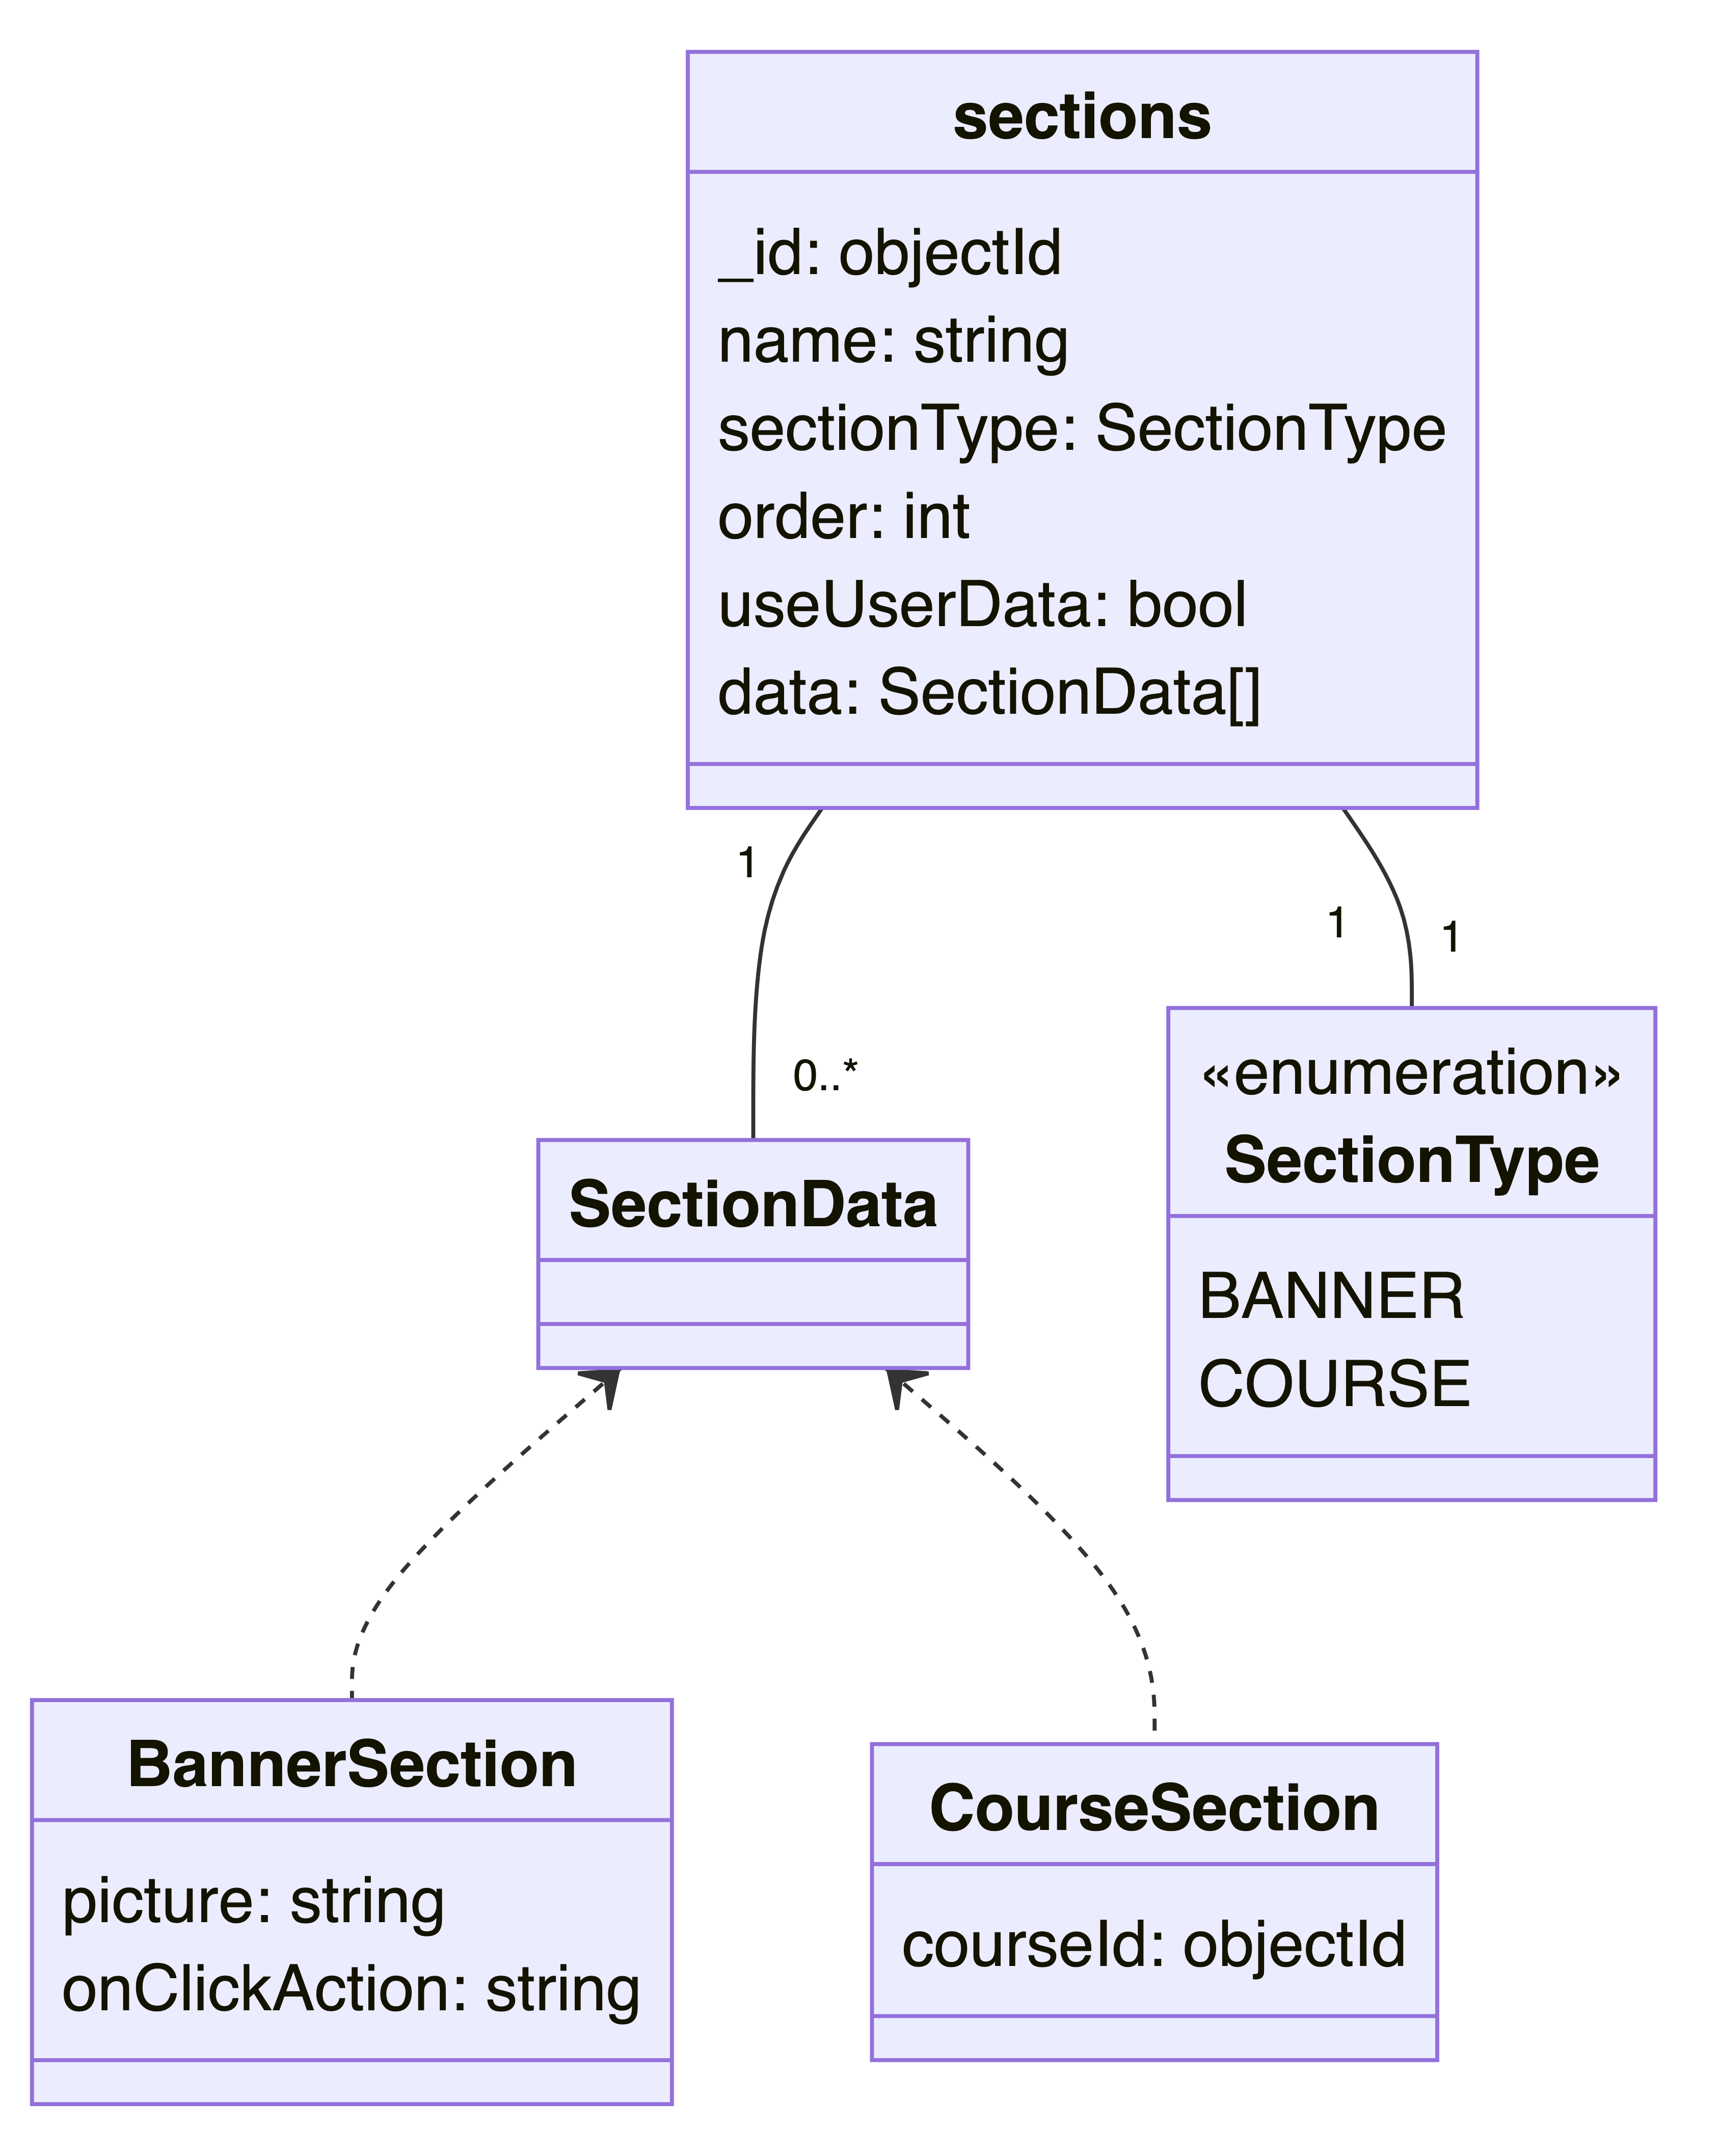
\includegraphics[width=9cm]{chapter_3/database/sections}
    \caption{แผนภาพยูสเคสในคอลเล็กชัน sections}
\end{figure}
\begin{table}
    \caption{รายละเอียดฐานข้อมูลในคอลเล็กชัน sections}
    \noindent ใช้ในการเก็บข้อมูลส่วนต่าง ๆ ในหน้าหลัก (Home) ที่จะมีการแนะนำคอร์สต่าง ๆ
    \begin{tabularx}{\textwidth}{ | l | l | X | }
        \hline
        \bf ชื่อแอตทริบิวต์ & \bf ชนิดตัวแปร & \bf รายละเอียด \\\hline
        \_id & objectId & ID ของส่วน\\\hline
        name & string & ชื่อของส่วนนี้\\\hline
        sectionType & SectionType & ประเภทของส่วน\\\hline
        order & int & ลำดับของส่วนบนหน้าหลัก\\\hline
        useUserData & bool & นำข้อมูลของผู้ใช้มาประกอบการแนะนำหรือไม่\\\hline
        data & SectionData[] & ข้อมูลของส่วน\\\hline
    \end{tabularx}
\end{table}

\begin{table}
    \caption{รายละเอียดชนิดคลาส BannerSection}
    \noindent ใช้ในการเก็บข้อมูลส่วนต่าง ๆ ในหน้าหลัก (Home) ที่จะมีการแนะนำคอร์สต่าง ๆ
    \begin{tabularx}{\textwidth}{ | l | l | X | }
        \hline
        \bf ชื่อแอตทริบิวต์ & \bf ชนิดตัวแปร & \bf รายละเอียด \\\hline
        picture & string & URL ไฟล์รูปภาพ\\\hline
        onClickAction & string & กำหนดการกระทำเมื่อผู้ใช้กดไปยัง Banner\\\hline
    \end{tabularx}
\end{table}

\begin{table}
    \caption{รายละเอียดชนิดคลาส CourseSection}
    \begin{tabularx}{\textwidth}{ | l | l | X | }
        \hline
        \bf ชื่อแอตทริบิวต์ & \bf ชนิดตัวแปร & \bf รายละเอียด \\\hline
        courseId & objectId & คอร์สที่แนะนำ\\\hline
    \end{tabularx}
\end{table}

\begin{table}
    \caption{รายละเอียด Enumeration SectionType}
    \begin{tabularx}{\textwidth}{ | l | X | }
        \hline
        \bf ชื่อแอตทริบิวต์ & \bf รายละเอียด \\\hline
        BANNER & ส่วนเป็นแบบ Banner\\\hline
        COURSE & ส่วนเป็นแบบ Course\\\hline
    \end{tabularx}
\end{table}
\subsection{ฐานข้อมูลในคอลเล็กชัน userFollowings}
\begin{figure}
    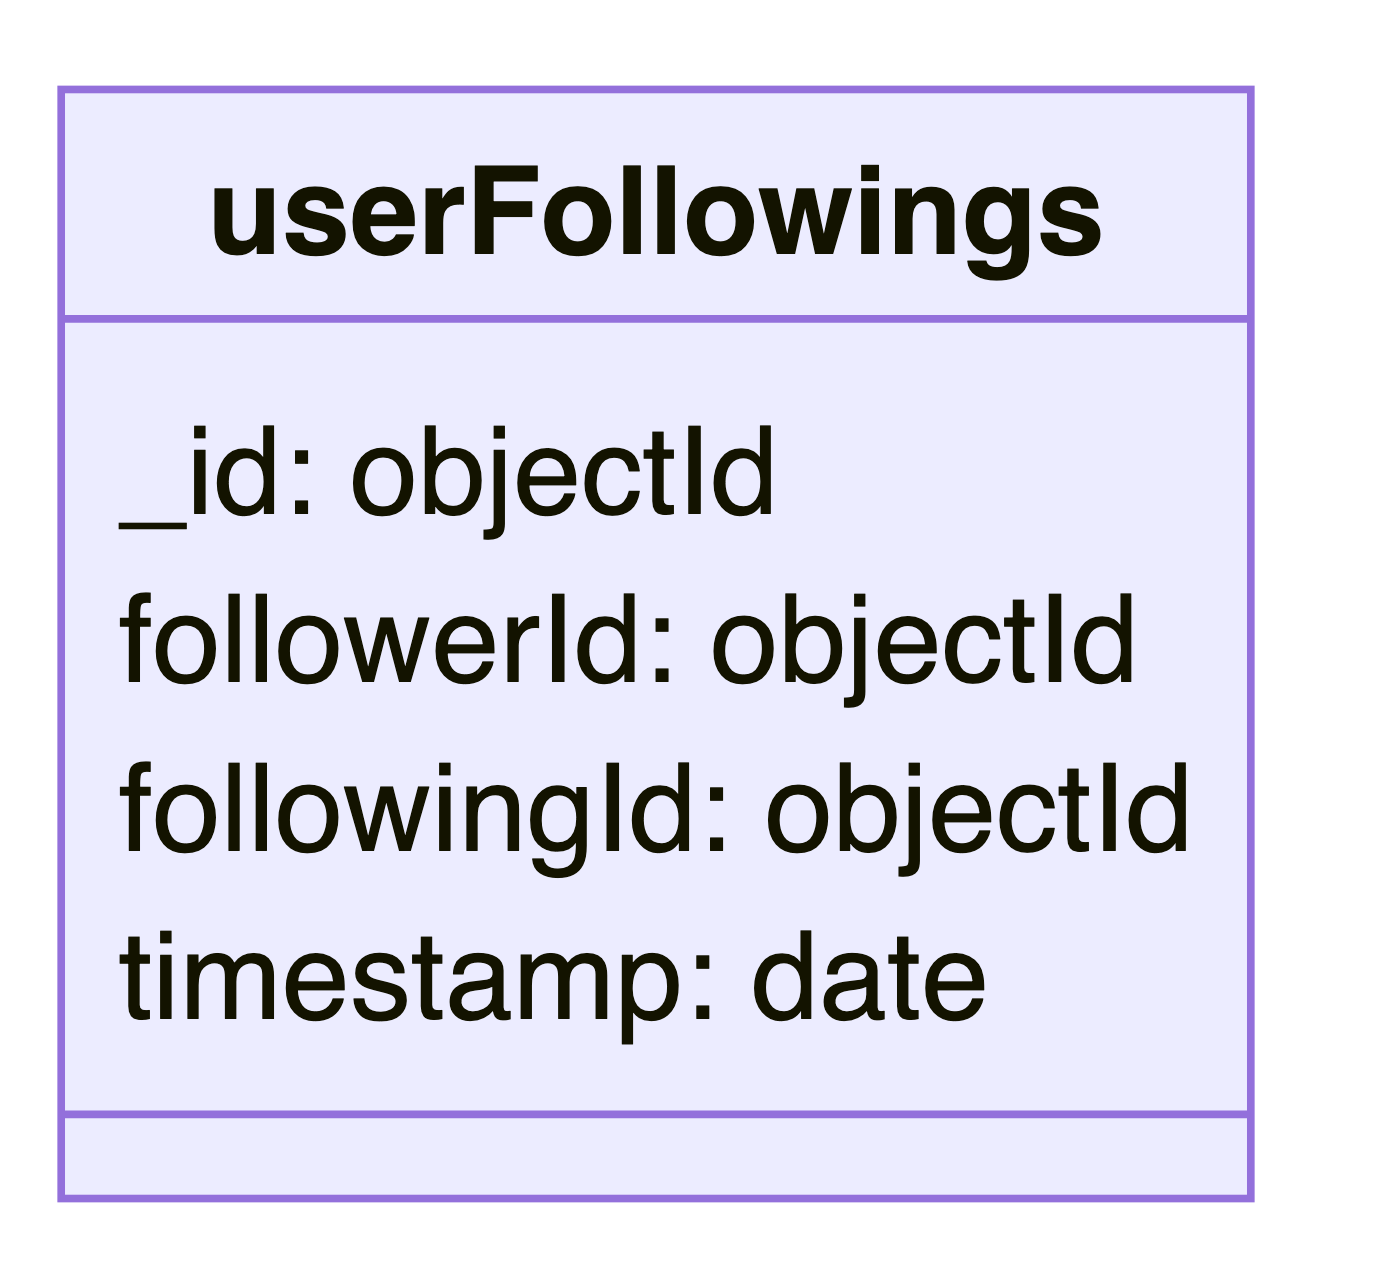
\includegraphics[width=5cm]{chapter_3/database/userFollowings}
    \caption{แผนภาพยูสเคสในคอลเล็กชัน userFollowings}
\end{figure}

\begin{table}
    \caption{รายละเอียดฐานข้อมูลในคอลเล็กชัน userFollowings}
    \begin{tabularx}{\textwidth}{ | l | l | X | }
        \hline
        \bf ชื่อแอตทริบิวต์ & \bf ชนิดตัวแปร & \bf รายละเอียด \\\hline
        \_id & objectId & ID ของรายการบันทึกการติดตามของผู้ใช้\\\hline
        followerId & objectId & ID ของผู้ใช้ที่กดติดตาม\\\hline
        followingId & objectId & ID ของผู้ใช้ที่ถูกติดตาม\\\hline
        timestamp & date & วันและเวลาที่ผู้ใช้ได้กดติดตาม\\\hline
    \end{tabularx}
\end{table}

\clearpage
